% Foliensatz: "AFu-Kurs nach DJ4UF" von DK0TU, Amateurfunkgruppe der TU Berlin
% Lizenz: CC BY-NC-SA 3.0 de (http://creativecommons.org/licenses/by-nc-sa/3.0/de/)
% Autoren: 
% Felix Baum DB4UM <baum@campus.tu-berlin.de>
% Lars Weiler DC4LW <dc4lw@darc.de>

preamble.dk0tu.tex
\subtitle{Technik Klasse A 03: \\
          Kondensator, Spule, Transformator \\[2em]}
\date{Stand 11.01.2016}
 \begin{document}

\begin{frame}
    \titlepage
    \vfill
    \begin{center}
        \ccbyncsaeu\\
        {\tiny This work is licensed under the \em{Creative Commons Attribution-NonCommercial-ShareAlike 3.0 License}.}\\[0.5ex]
         \tiny Amateurfunkgruppe der Technische Universität Berlin (AfuTUB), DKØTU
         %\includegraphics[scale=0.5]{img/DK0TU_Logo.pdf}
    \end{center}
\end{frame}


\section*{Einleitung}

\begin{frame}
    \frametitle{Einleitung / Kondensator}
    \begin{center}
        \Large{Wofür nutzen?}\\
        \Large{Wichtige Merkmale?}         
    \end{center}
\end{frame}

\begin{frame}
  \frametitle{Einleitung / Kondensator}
  \begin{block}{Ladung und Kapazität}
    \begin{center}
      \Large{$Q = C \cdot U$}\\
      \Large{$C= \varepsilon_{0} \cdot \varepsilon_{r} \cdot \frac{A}{d}$}
    \end{center}
  \end{block}
  \begin{center}
    \includegraphics[width=0.9\textwidth,height=0.6\textheight,keepaspectratio]{e05/Kondensator02.jpg}
    \tiny \hyperlink{refs}{\cite{wc}}
  \end{center}
\end{frame}


\begin{frame}
    \frametitle{Einleitung / Spule}
    \begin{center}
        \Large{Wofür nutzen?}\\
        \Large{Wichtige Merkmale?}         
    \end{center}
\end{frame}

\begin{frame}
  \frametitle{Einleitung / Spulen-Beispiele}
  \begin{block}{Induktivität}
    \begin{center}
      \Large{$L = \cfrac{\mu_0 \cdot \mu_r \cdot N^2 \cdot A_S}{\ell_m}$}
    \end{center}
  \end{block}
  \begin{center}
    \includegraphics[width=0.6\textwidth,height=0.5\textheight,keepaspectratio]{a03/Spule.jpg}
    \footnote{\tiny \url{https://commons.wikimedia.org/wiki/File:Electronic_component_inductors.jpg}}
  \end{center}
\end{frame}


\section*{Laden und Entladen}

\begin{frame}
    \frametitle{Kondensator Laden}
    \begin{center}
        \Large{Mit welcher Kurve lädt sich der Kondendsator auf?}\\        
    \end{center}
\end{frame}

\begin{frame}
    \frametitle{Kondensator Spannung}
	\begin{center}
        \includegraphics[width=1\textwidth,height=.85\textheight,keepaspectratio]{a03/Capacitor_Charge_Graph.jpg}
        \tiny \hyperlink{refs}{\cite{wc}}
    \end{center}
\end{frame}

\begin{frame}
    \frametitle{Kondensator an Rechteckspannung}
	\begin{center}
        \includegraphics[width=1\textwidth,height=.85\textheight,keepaspectratio]{a03/Capacitor_Square_wave_charge-discharge.png}
                \tiny \hyperlink{refs}{\cite{wc}}
    \end{center}
\end{frame}

\begin{frame}
    \frametitle{Kondensator Strom beim Laden}
	\begin{center}
        \includegraphics[width=1\textwidth,height=.75\textheight,keepaspectratio]{a03/Ladevorgang.png}
                \tiny \hyperlink{refs}{\cite{wc}}\\
        \Large{Je stärker die Spannungsänderung, desto mehr Strom fließt.}
    \end{center}
\end{frame}

\begin{frame}
    \frametitle{Kondensator Strom beim Laden}
	\begin{center}
        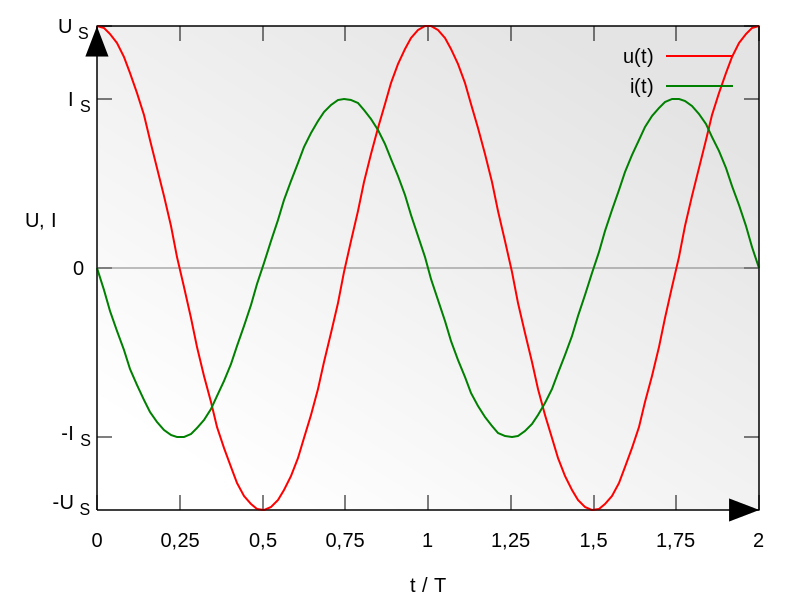
\includegraphics[width=1\textwidth,height=.85\textheight,keepaspectratio]{a03/Sinus_Voltage_and_Current_of_a_Capacitor.png}
        \tiny \hyperlink{refs}{\cite{wc}}
    \end{center}
\end{frame}

\begin{frame}
\frametitle{Merksatz Kondensator}
  \begin{block}{Merksatz}
    Kondensator:\\
    Strom eilt vor
  \end{block}
\end{frame}

\begin{frame}
    \frametitle{Wie verhält sich diese Schaltung?}
	\begin{center}
        \includegraphics[width=.8\textwidth,height=.85\textheight,keepaspectratio]{a03/Spulenstrom.png}
        \tiny \hyperlink{refs}{\cite{wc}}
    \end{center}
\end{frame}

\begin{frame}
	\frametitle{Spule}
\begin{minipage}{0.45\textwidth}
	\includegraphics[width=.95\textwidth,height=.85\textheight,keepaspectratio]{a03/Spulenstrom.png}
	\tiny \hyperlink{refs}{\cite{wc}}
\end{minipage}
\begin{minipage}{0.5\textwidth}
	\includegraphics[width=.95\textwidth,height=.85\textheight,keepaspectratio]{a03/Selbstinduktion-im-gleichstromkreis-zeitverlauf.png}
	\tiny \hyperlink{refs}{\cite{wc}}
\end{minipage}
\end{frame}

\begin{frame}
    \frametitle{Phasenverschiebung Spule}
	\begin{center}
        \includegraphics[width=1\textwidth,height=.85\textheight,keepaspectratio]{a03/Phasenverschiebung_induktiv.png}
        \tiny \hyperlink{refs}{\cite{wc}}
    \end{center}
\end{frame}

\begin{frame}
  \frametitle{Merksatz Spule}
  \begin{block}{Merksatz}
    Bei Induktivitäten,\\
    Ströme sich verspäten.
  \end{block}
\end{frame}

\begin{frame}
  \frametitle{Merksatz Widerstand}
  \begin{block}{Merksatz}
    Beim reinen Ohmschen Widerstand\\
    gehn Strom und Spannung Hand in Hand
  \end{block}
\end{frame}

\section*{Komplexer Widerstand}

\begin{frame}
  \frametitle{Blindwiderstand}
  \begin{columns}
    \column{0.45\textwidth}
    \begin{block}{Kondensator}
      \begin{center}
	\huge{$X_{C} = \frac{1}{\omega C}$}
      \end{center}
    \end{block}
    
  \column{0.45\textwidth}
    \begin{block}{Spule}
      \begin{center}
	\huge{$X_{L} = \omega L$}
      \end{center}
    \end{block}
  \end{columns}

  \begin{center}
    \vspace{1cm}
    Was war nochmal $\omega$? \\
  \end{center}
\end{frame}

\begin{frame}
\frametitle{Komplexer Widerstand}
Für E-Techniker, aber nicht für die Amateurfunkprüfung relevant.
\begin{center}
		\includegraphics[width=.8\textwidth,height=.5\textheight,keepaspectratio]{a03/Widerstand_Zeiger.png}
		{\tiny \hyperlink{refs}{\cite{wc}}}
\begin{block}{Für den Gesamtwiderstand gilt}
$Z = R + jX$ \\
$|Z| = \sqrt{R^2 + X^2}$
\end{block}
\end{center}
\end{frame}
	
\begin{frame}
\frametitle{Elko Ersatzschaltbild}
\begin{center}
		\includegraphics[width=.8\textwidth,height=.4\textheight,keepaspectratio]{a03/Elko-Ersatzschaltbild.png}
		{\tiny\hyperlink{refs}{\cite{wc}}\\
		nach DIN EN 60384-1 vom Februar 2002} \\[1em]

        $R_{Leak}$ $\rightarrow$ Leckströme am Elko\\
        $R_{ESR}$ $\rightarrow$ ohmsche Verluste des Bauelementes\\
        $L_{ESL}$ $\rightarrow$ Induktivität des Bauelementes\\
        Verlustfaktor $tan \delta$ $\rightarrow$ Angabe in alten Datenblättern \\im Bezug auf ESR ($\omega C \cdot$ ESR $= tan \delta$)
\end{center}
\end{frame}
	

\section*{Reihen- und Parallelschaltung}

\begin{frame}
  \frametitle{Reihen- und Parallelschaltung von Kondensatoren}
  \begin{center}
    \huge Wie war noch einmal die Formel für die Reihen- und Parallelschaltung von Kondensatoren?
  \end{center}
\end{frame}
 
\begin{frame}
  \frametitle{Reihen- und Parallelschaltung von Kondensatoren}	
  \begin{block}{Parallelschaltung von Kondensatoren}
    \begin{center}
      \huge{$C_{ges} = C_{1} + C_{2} + C_{3} + C_{4} + C_{5} + \cdots$} 
    \end{center}
  \end{block}
  \pause
  \begin{block}{Reihenschaltung von Kondensatoren}
    \begin{center}
      \huge{$\frac{1}{C_{ges}} = \frac{1}{ C_{1}} + \frac{1}{C_{2}} + \frac{1}{C_{3}} + \frac{1}{C_{4}} + \frac{1}{C_{5}} + \cdots$}
    \end{center}
  \end{block}
\end{frame}
    
\begin{frame}
  \frametitle{Reihen- und Parallelschaltung von Spulen}
  \begin{center}
    \huge Wie war noch einmal die Formel für die Reihen- und Parallelschaltung von Spulen?
  \end{center}
\end{frame}

\begin{frame}
  \frametitle{Reihen- und Parallelschaltung von Spulen}
  \begin{block}{Reihenschaltung von Spulen}
    \begin{center}
      \huge{$L_{gesamt} = L_1 + L_2 + L_3 + \cdots$}
    \end{center}
  \end{block}
  \pause
  \begin{block}{Parallelschaltung von Spulen}
    \begin{center}
      \huge{$\frac{1}{L_{gesamt}} = \frac{1}{L_1} + \frac{1}{L_2} + \frac{1}{L_3} + \cdots$}
    \end{center}
  \end{block}
\end{frame}

\section*{Induktivitäten mit Kern}

\begin{frame}
  \frametitle{Spule mit Kern}
  \begin{center}
    Für große Induktivitäten werden die Spulen um einen Kern gewickelt.\\
    Wichtiger Wert dafür ist der Kernfaktor $A_{L}$ (immer im Datenblatt)
    \begin{block}{Induktivität von Schalenkernspulen}
      \huge	$$L = N^2 \cdot A_{L}$$
    \end{block}
  \end{center}
\end{frame}

\section*{Transformator}
\begin{frame}
  \frametitle{Transformator}
  \begin{center}
    \includegraphics[width=0.9\textwidth,height=.8\textheight,keepaspectratio]{a03/trafo-Real.jpg}
    \footnote{\tiny \url{https://commons.wikimedia.org/wiki/File:Trafo_6.jpg}}
  \end{center}
\end{frame}

\begin{frame}
  \frametitle{Transformator}
  \begin{block}{Übersetzungsverhältnis}
    $$\text{\"u} = \frac{N_P}{N_S} = \frac{U_P}{U_S} $$
  \end{block}
  \vspace{2em}
  \begin{block}{Übersetzungsverhältnis von Strom und Spannung}
    \begin{align*}
    P_P &= P_S\\
    \Rightarrow U_{P} \cdot I_P &= U_{S} \cdot I_S\\
    \Rightarrow \frac{U_P}{U_S} &= \frac{I_S}{I_P}
  \end{align*}
  \end{block}
\end{frame}

\begin{frame}
  \frametitle{Widerstandsanpassung}
  \begin{block}{Impedanzanpassung}
    $$\text{\"u} = \frac{N_P}{N_S} = \sqrt{\frac{Z_P}{Z_S}}$$
  \end{block}
  \vspace{2em}
  Wird benötigt, wenn z.B. der Fußpunktwiderstand einer Antenne bei $200\Omega$ liegt, aber mit einem $50\Omega$ Coaxkabel gespeist werden soll.
\end{frame}

\section*{Balun}

\begin{frame}
    \frametitle{Balun Theorie}
	\begin{center}
        \includegraphics[width=0.8\textwidth,height=.85\textheight,keepaspectratio]{a03/Cdbalun2.png}
                \tiny \hyperlink{refs}{\cite{wc}}
    \end{center}
\end{frame}

\begin{frame}
    \frametitle{Balun Real}
	\begin{center}
        \includegraphics[width=0.9\textwidth,height=.85\textheight,keepaspectratio]{a03/balun-Real.jpg}
                \tiny \hyperlink{refs}{\cite{wc}}
    \end{center}
\end{frame}


\renewcommand{\refname}{Referenzen}

\hypertarget{refs}{}
\textcolor{white}{} \\ %\vspace{} geht nicht
\Large Referenzen/Links
\footnotesize

\begin{thebibliography}{}
    \bibitem{dj4uf} Moltrecht A 03: \\
                    \url{http://www.darc.de/referate/ajw/ausbildung/darc-online-lehrgang/technik-klasse-a/technik-a03/}

    \bibitem{wc}    Wikimedia Commons: \\
                    \url{https://commons.wikimedia.org/wiki/File:Sinus_Voltage_and_Current_of_a_Capacitor.svg}\\
                    \url{https://commons.wikimedia.org/wiki/File:Selbsti.gif}\\
                    \url{https://commons.wikimedia.org/wiki/File:Selbstinduktion-im-gleichstromkreis-zeitverlauf.svg}\\
                    \url{http://commons.wikimedia.org/wiki/File:Capacitors_(7189597135).jpg}\\
                    \url{https://commons.wikimedia.org/wiki/File:Phasenverschiebung_induktiv.svg}\\
                    \url{https://commons.wikimedia.org/wiki/File:Widerstand_Zeiger.svg}\\
                    \url{https://commons.wikimedia.org/wiki/File:Elko-Ersatzschaltbild-Wiki-07-02-08.svg}\\
                    \url{https://commons.wikimedia.org/wiki/File:T200A2.jpg}\\
                    \url{https://commons.wikimedia.org/wiki/File:Cdbalun2.svg}\\
\end{thebibliography} 

% Hier könnte noch eine Kontaktfolie stehen

\end{document}

